% !TEX encoding = UTF-8
% !TEX program = xelatex
\documentclass[12pt,a4paper]{article}
\usepackage[paperwidth=210mm, paperheight=297mm, left=0.75in, right=0.75in, bottom=1in, top=1in]{geometry}
\usepackage{polyglossia}
\setdefaultlanguage[babelshorthands]{italian}
\usepackage{fontspec}
\usepackage{graphicx}
\usepackage{blindtext}
\usepackage{wrapfig}

\frenchspacing
\makeindex

\begin{document}
\title{\vspace{-70pt}Voyager 1}
\author{Patrick Predella}
\date{}
\maketitle
\pagestyle{empty}
\thispagestyle{empty}

\section*{Storia}
\label{storia}
\begin{wrapfigure}{r}{0.35\textwidth}
  \vspace{-10pt}
  \begin{center}
    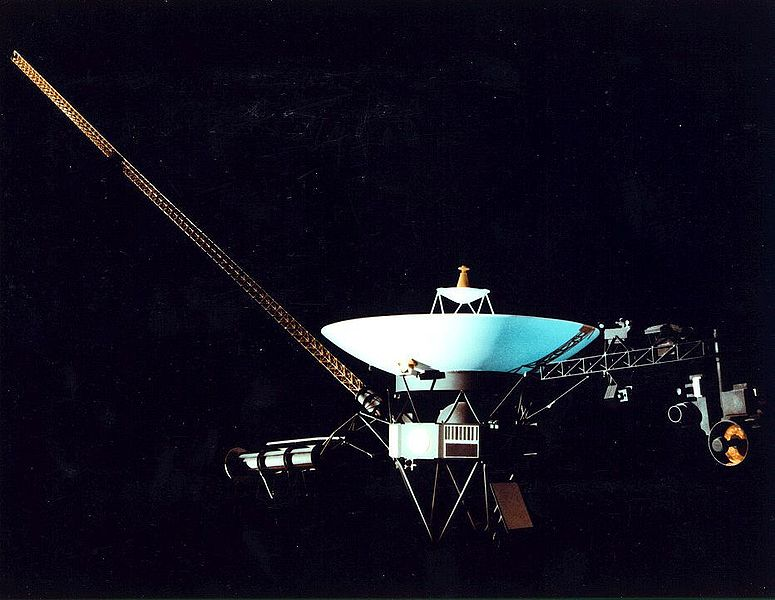
\includegraphics[width=0.30\textwidth]{satellite}
  \end{center}
  \vspace{-20pt}
\end{wrapfigure}
La sonda Voyager 1 fa parte del programma Voyager insieme alla sonda sorella Voyager 2. È partita il 5 settembre 1977 con un razzo vettore \emph{Titan 3} e aveva come missione primaria quella di effettuare un volo tra Saturno e Giove grazie ad un allineamento vantaggioso dei 2 pianeti. È tutt'ora in attività, anche se non tutta la strumentazione è funzionante.
Grazie ad essa abbiamo numerosissime informazioni, sia sotto forma di rilevamenti chimici che di fotografie. Le due sonde vennero usate per porre fine alla teoria di un pianeta post-plutoniano.
Recentemente Voyager 1 ha superato i margini più estremi dell' eliopausa, dove le particelle solari vengono rallentate fino a velocità zero, e si sta dirigendo verso l'esterno del sistema solare. 

\section*{Osservazioni}
\label{osservazioni}

La Voyager 1 iniziò a fotografare Giove nel gennaio 1979. La sonda passò vicino a Giove il 5 marzo 1979, e continuò a fotografare il pianeta fino ad aprile. Poco tempo dopo fu la volta della sonda sorella Voyager 2. Le due Voyager fecero numerose scoperte su Giove e i suoi satelliti. La più sorprendente fu la scoperta di vulcani di zolfo su Io, che non erano mai stati osservati né da Terra né dal Pioneer 10 o dal Pioneer 11.
La sonda proseguì il suo viaggio verso Saturno. Il punto di massimo avvicinamento fu raggiunto il 12 novembre 1980, quando passò ad una distanza di poco più di 120 000 km dal pianeta. La sonda fotografò le complesse strutture degli anelli di Saturno, e studiò l'atmosfera di Saturno e di Titano. La sua orbita, progettata per studiare Titano da vicino, la portò fuori dal piano dell'eclittica, impedendole di visitare altri pianeti. Da allora si sta allontanando dal sistema solare.
Dati recenti del dicembre 2012 inviati dalla sonda dimostrano nuove e sensazionali scoperte dei confini del sistema solare.

\section*{Curiosità}
\label{curiosit}

Voyager 1 è attualmente il oggetto costruito dall'uomo più distante dalla terra infatti si sta dirigendo verso lo spazio interstellare. si chiama Voyager 1 anche se venne lanciata dopo la Voyager 2.
La sonda Voyager trasporta un disco di rame e oro che contiene immagini e suoni della terra, con il codice per decriptarlo scritto sopra.
Fa parte di un progetto iniziato da Carl Sagan.
Viene inserito in modo provocatorio nel film star trek del 1979, come oggetto che ha raccolto tante informazioni da diventare autonomo, ma che cerca il creatore. Essa non viene riconosciuta a causa del nome V'ger.

\end{document}